\begin{flushleft}
Il codice seguente:
\lstinputlisting[language=Matlab]{cap_1/es4/es4.m}
restituisce questo risultato (assumendo che $f(x)$ = $ e^x $ e $ x_0 = 0 $ ): 
\begin{center}
\begin{tabular}{|c|c|}
\hline
h & \( \Psi_{h}(0) \)  \\
\hline
    \(10^{-1}\) & 1.051709180756477e+00\\
    \(10^{-2}\) & 1.005016708416795e+00\\
    \(10^{-3}\) & 1.000500166708385e+00\\
    \(10^{-4}\) & 1.000050001667141e+00\\
    \(10^{-5}\) & 1.000005000006965e+00\\
    \(10^{-6}\) & 1.000000499962184e+00\\
    \(10^{-7}\) & 1.000000049433680e+00\\
    \(10^{-8}\) & 9.999999939225290e-01\\
    \(10^{-9}\) & 1.000000082740371e+00\\
    \(10^{-10}\) & 1.000000082740371e+00\\
    \(10^{-11}\) & 1.000000082740371e+00\\
    \(10^{-12}\) & 1.000088900582341e+00\\
\hline
\end{tabular} \\
\end{center}
Si vede che i valori di $\Psi_{h}(0)$ diminuiscono fino ad $h = 10^{-8}$, in cui si ha il minimo valore di $\Psi_{h}(0)$, dopodichè l'errore inizia a crescere. Mostriamo l'andamento relativo nel seguente plot:
\begin{figure}[H]
\label{fes14}
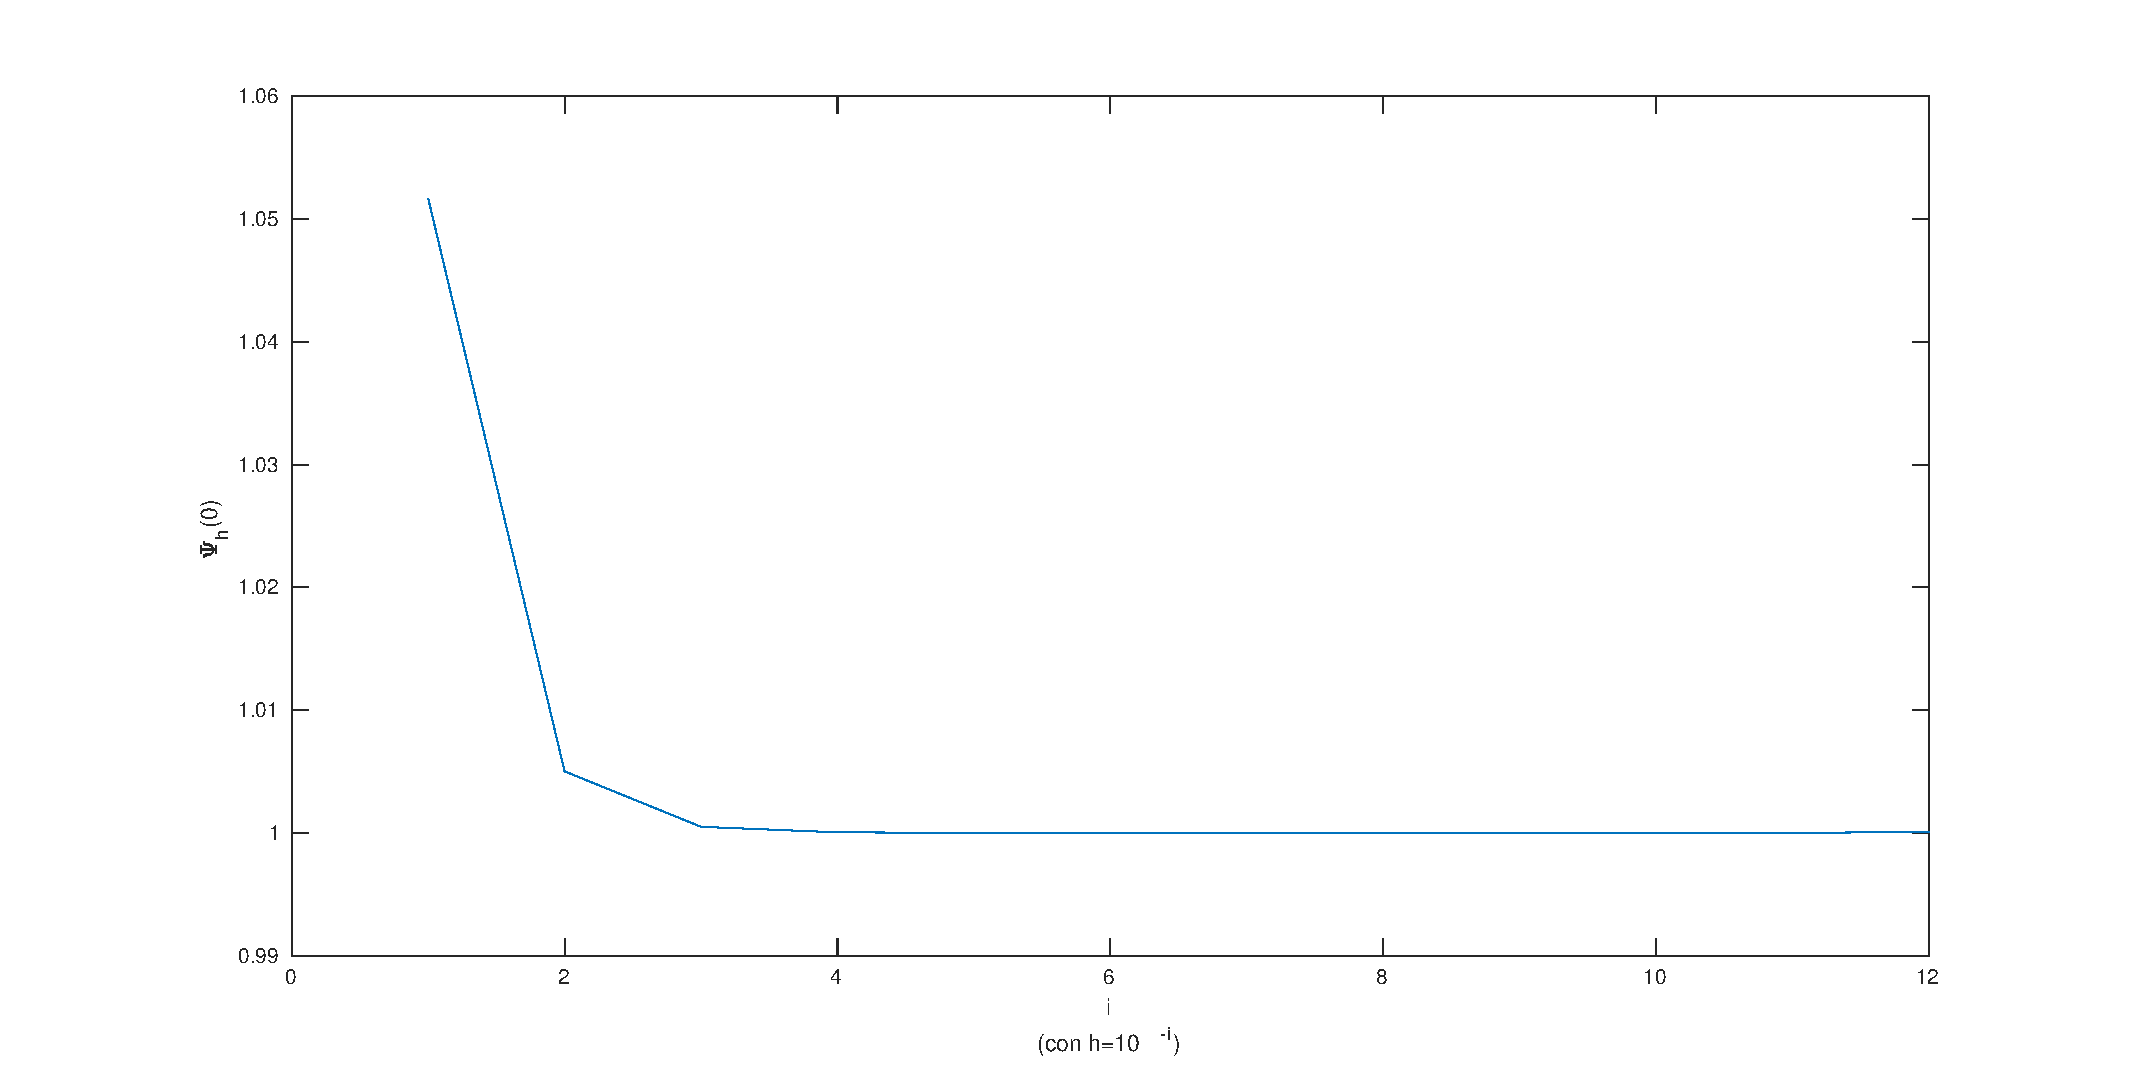
\includegraphics[left, width=200px]{plot/fes14}
\caption{Andamento della funzione $\Psi_{h}(0)$}
\end{figure}
\end{flushleft}